En esta tercer pra\'ctica comenzaremos a trabajar con operaciones matem\'aticas
entre las bandas y relacionaremos los resultados con variables biof\'isicas medibles en el terreno. Son
nuestros objetivos:

\begin{itemize}
    \item Calcular los \'indices de vegetaci\'on a partir de las im\'agenes en
        reflectancia.
    \item Calcular la l\'inea de suelo como par\'ametro para obtener \'indices
        de vegetaci\'on.
    \item Realizar modelos emp\'iricos que relacionen variables biof\'isicas
        medidas a campo con los \'indices espectrales.
    \item Construir mapas a partir de los modelos emp\'iricos antes mencionados.
\end{itemize}


\section{C\'alculo de \'indices entre bandas}
Utilizaremos las librerias \texttt{raster} y \texttt{RStoolbox}. Para
poder usar mejores paletas de colores utilizaremos la libreria
\texttt{RColorBrewer}. Por \'ultimo, puede ayudar cargar la libreria \texttt{rasterVis}
para realizar algunos de los gr\'aficos.

Comenzamos primero cargando la imagen desde el metadato y convirti\'endola a
reflectancia entre cero y uno.

\begin{lstlisting}
    xml.2016 <- readMeta("raster_data/LC82240782016304/LC82240782016304LGN00.xml")
    ref.2016 <- stackMeta(xml.2016, quantity = "sre")
    scaleF <- getMeta(ref.2016,xml.2016, what = "SCALE_FACTOR")
    ref.2016 <- ref.2016 * scaleF
    ref.2016 <- ref.2016[[-1,]]
    names(ref.2016) <- c("blue","green","red","nir","swir1","swir2")
\end{lstlisting}

Luego podemos realizar operaciones entre las bandas llamando
a cada una por separado. Veamos como ejemplo el calculo de NDVI\@.

\begin{exa}
    C\'alculo de NDVI a mano.
    \begin{lstlisting}
    ndvi.2016 <- (ref.2016$nir-ref.2016$red)/(ref.2016$nir+ref.2016$red)
    cols = colorRampPalette(brewer.pal(9,"YlGn"))(256)
    plot(ndvi.2016, col=cols, zlim = c(0,1))
    \end{lstlisting}
    En este caso estamos
    \begin{itemize}
        \item Calculando el NDVI a mano usando la formula $(\rho_n-\rho_r)/(\rho_n+\rho_r)$.
        \item Obteniendo una rampa de color entre amarillo y verde.
        \item Graficando el NDVI, usamos como colores la rampa anterior
            y ajustandolo entre 0 y 1, es decir, los valores menores a 0 se
            mostrar\'an todos del mismo color.
    \end{itemize}
    Obtenemos entonces el resultado de la figura \ref{fig:ndvifig}
    \begin{figure}[h!]
    \begin{center}
        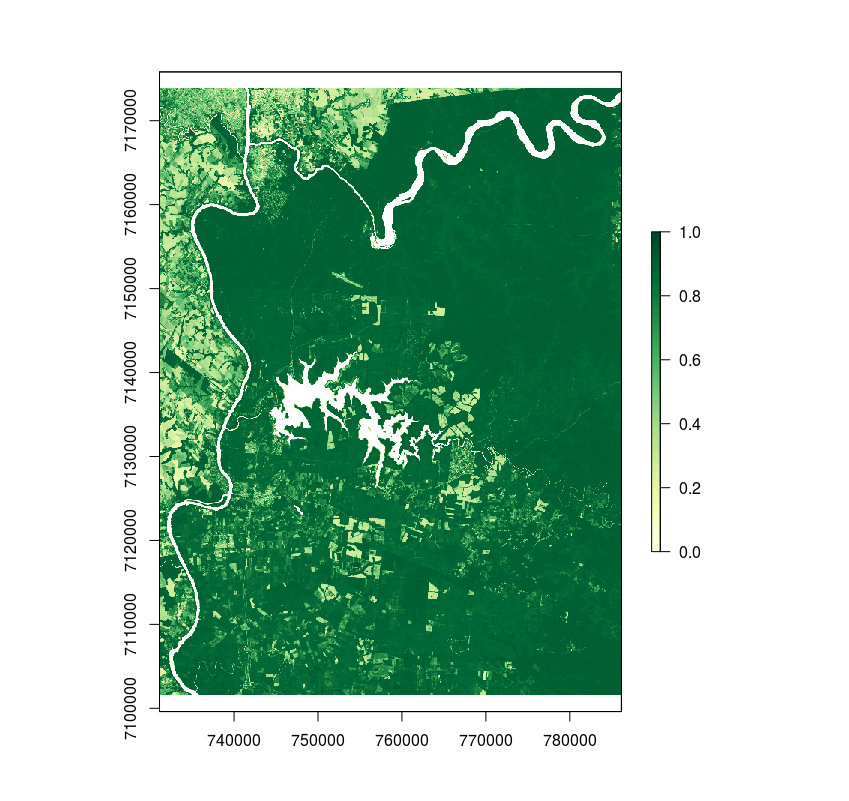
\includegraphics[scale=0.6]{ndvi_fig.png}
    \end{center}
    \caption{Mapa del NDVI en escala de verdes.}
    \label{fig:ndvifig}
    \end{figure}

\end{exa}

El paquete \texttt{RStoolbox} tiene varias herramientas que nos ayudan a
calcular los \'indices espectrales. Veamos por ejemplo como calcular el NDVI y el
EVI.

\begin{exa}
    Para calcular los \'indices mediante la funci\'on \texttt{spectralIndices} debemos
    especificar con que raster trabajamos y que bandas corresponden a cada
    longitud de onda
    \begin{lstlisting}
    indices.2016 <- spectralIndices(ref.2016,
                                    blue="blue", red="red", nir="nir",
                                    indices=c("NDVI","EVI"))
    plot(indices.2016,col=cols, zlim=c(0,1))
    \end{lstlisting}
    En este caso, vemos que la funci\'on \texttt{espectralIndices} necesita al
    menos 3 par\'ametros
    \begin{itemize}
        \item Una imagen.
        \item A que zona del espectro corresponde cada banda.
        \item Los \'indices que queremos calcular
    \end{itemize}
     \begin{figure}[h!]
     \begin{center}
         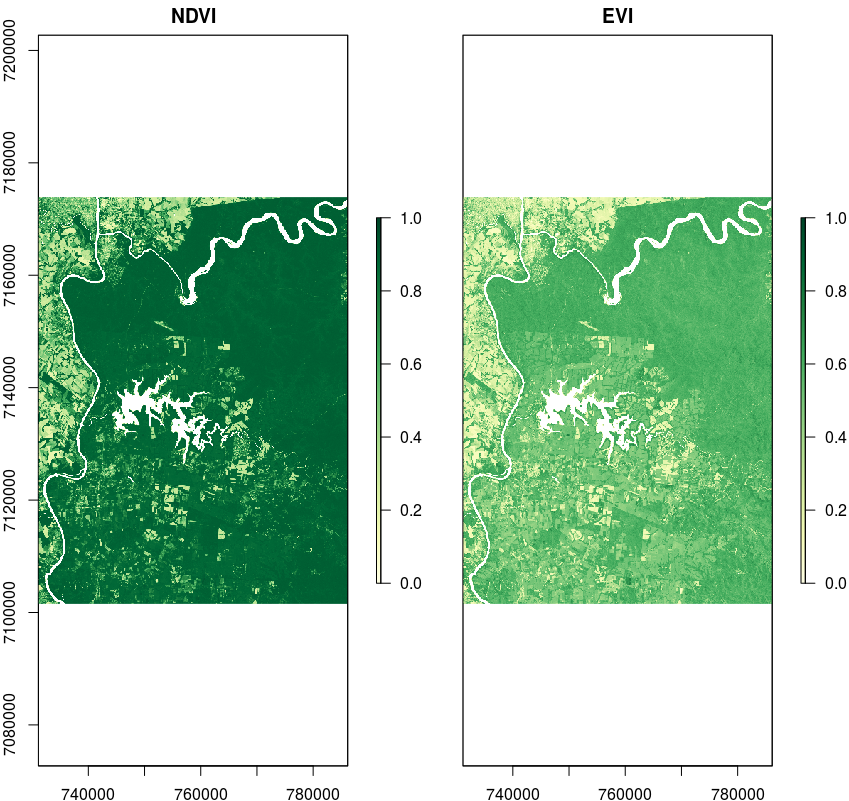
\includegraphics[scale=0.6]{evi-ndvi.png}
     \end{center}
     \caption{Graficos del EVI y el NDVI para la imagen seleccionada.}
     \label{fig:evi-ndvi}
     \end{figure}

\end{exa}

\begin{act}
    Calcule el NDVI y el EVI para el año 2000 utilizando la imagen landsat 7.
\end{act}

\begin{act}
    Calcule y grafique todos los \'indices posibles que involucren a las bandas
    roja e infrarrojo cercano de Landsat 8. Puede ayudarse con el comando
    \texttt{?spectralIndices}.
\end{act}

\section{C\'alculo de la l\'inea de suelo}

La l\'inea de suelo es una cantidad que definimos en teledetecci\'on que aporta
informaci\'on sobre las imagen que estamos analizando y sirve para incorporar
los efectos de la reflectancia del suelo en el c\'alculo de \'indices.
Veamos como hacerlo con la libreria \texttt{landsat}

\begin{exa}
    Calculemos la l\'inea de suelo a partir de la imagen Landsat 8.
    Para esto necesitamos enmascarar las zonas con
    cobertura de agua y nubes.
    \begin{lstlisting}
    mask.2016 <- raster("raster_data/LC82240782016304/LC82240782016304LGN00_cfmask.tif")
    masked.2016 <- mask(ref.2016, mask=mask.2016, inverse=TRUE,
                        maskvalue=0, updatevalue=255)
    masked.2016[masked.2016<=0] <- 255
    \end{lstlisting}
    de esta forma enmascaramos todos los valores con nubes, agua y donde la
    reflectancia obtenida es cero con el valor 255.
    Calculamos ahora la l\'inea de suelo y la mostramos en un scatterplot
    \begin{lstlisting}
    bsl.2016 <- BSL(as.matrix(masked.2016$red), as.matrix(masked.2016$nir),
                    method="quantile")
    plot(ref.2016$red, ref.2016$nir)
    abline(bsl.2016$BSL,col="red")
    \end{lstlisting}
    Obtenemos como resultado el gr\'afico de (Figura \ref{fig:soil}). Podemos consultar
    los demas par\'ametros imprimiendo la variable \texttt{bsl.2016}.
    \begin{figure}[h!]
    \begin{center}
        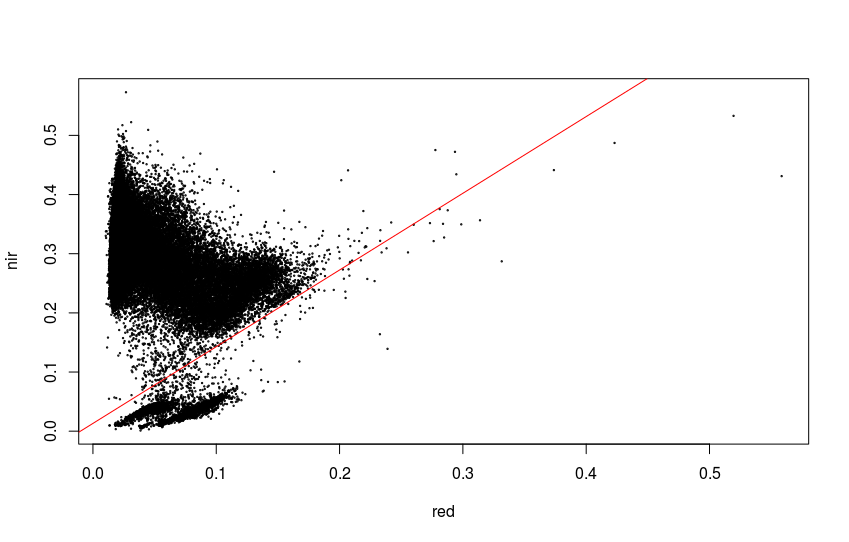
\includegraphics[scale=0.6]{soil.png}
    \end{center}
    \caption{L\'inea de suelo sobre el scatterplot nir-red}
    \label{fig:soil}
    \end{figure}

\end{exa}

\begin{act}
    Calcule el tSAVI utilizando la l\'inea de suelo.
\end{act}

\begin{act}
    Calcule la l\'inea de suelo sin enmascarar la imagen y dibuje el
    scatterplot conto con ella.
\end{act}

\begin{act}
    Obtenga la l\'inea de suelo y calcule el \'indice tSAVI para la imagen del año
    2000.
\end{act}

\section{Estimaci\'on de par\'ametros biof\'isicos}

Finalmente, veamos como se puede obtener datos biof\'isicos a partir de los
\'indices de vegetaci\'on para realizar mapas de
porcentaje de cobertura, productividad, etc.

\begin{exa}
    Comenzamos calculando el NDVI para el año 2016, y utilizando la capa
    muestreo, hacemos una extracci\'on estadi\'stica sobre la misma.
    \begin{lstlisting}
    vector <- readOGR(dsn="vector_data/", layer="muestreo")
    datos <- extract(ndvi.2016,vector)
    DF <- data.frame(vector@data,datos)
    pairs(DF)
    \end{lstlisting}

    Obtendremos un gr\'afico que presenta los scatterplots entre las bandas, su
    correlaci\'on e histogramas.
    Vemos que la superficie cubierta por vegetaci\'on var\'ia
    linealmente con el NDVI\@. Por lo tanto, los utilizaremos para hacer un ajuste de nuestro modelo

    \begin{lstlisting}
        lm.2016 <- lm(fcover~ndvi, data=muestreo)
        plot(muestreo$ndvi, mustreo$fcover)
        abline(lm.2016, col="red")
        summary(lm.2016)
    \end{lstlisting}

    de esta forma obtenemos los par\'ametros de nuestro ajuste.

    Para aplicar el modelo a nuestro raster hacemos
    \begin{lstlisting}
        fcover.2016 <- predict(ndvi.2016,lm.2016)
        plot(fcover.2016)
    \end{lstlisting}
\end{exa}

\begin{act}
    Genere los modelos de lai, fapar y fcover para el año 2016 y
    realice mapas de dichas variables.
\end{act}

\begin{act}
    Utilizando los modelos obtenidos para 2016 realice
    los mapas de lai, fapar y fcover del año 2000. ¿Que suposici\'on est\'a
    haciendo? Compare distintas zonas de los modelos en el qgis.
\end{act}
